\documentclass{article}

% Packages for formatting
\usepackage[margin=1in]{geometry}
\usepackage{fancyhdr}
\usepackage{enumerate}
\usepackage{graphicx}
\usepackage{kotex}
\usepackage{amsmath}
\usepackage{amsthm}
\usepackage{algorithm2e,setspace}
\usepackage{algpseudocode}
\usepackage{xcolor}
\usepackage{amssymb}

% Fonts
\usepackage[T1]{fontenc}
\usepackage[utf8]{inputenc}
\usepackage{newpxtext,newpxmath}
\usepackage{sectsty}

% Define colors
\definecolor{blue1}{HTML}{0077c2}
\definecolor{blue2}{HTML}{00a5e6}
\definecolor{blue3}{HTML}{b3e0ff}
\definecolor{blue4}{HTML}{00293c}
\definecolor{blue5}{HTML}{e6f7ff}

\definecolor{thmcolor}{RGB}{231, 76, 60}
\definecolor{defcolor}{RGB}{52, 152, 219}
\definecolor{lemcolor}{RGB}{155, 89, 182}
\definecolor{corcolor}{RGB}{46, 204, 113}
\definecolor{procolor}{RGB}{241, 196, 15}

\usepackage{color,soul}
\usepackage{soul}
\newcommand{\mathcolorbox}[2]{\colorbox{#1}{$\displaystyle #2$}}
\usepackage{cancel}
\newcommand\crossout[3][black]{\renewcommand\CancelColor{\color{#1}}\cancelto{#2}{#3}}
\newcommand\ncrossout[2][black]{\renewcommand\CancelColor{\color{#1}}\cancel{#2}}

\usepackage{hyperref}
\usepackage{booktabs}

% Chapter formatting
\definecolor{titleblue}{RGB}{0,53,128}
\usepackage{titlesec}
\titleformat{\section}
{\normalfont\sffamily\Large\bfseries\color{titleblue!100!gray}}{\thesection}{1em}{}
\titleformat{\subsection}
{\normalfont\sffamily\large\bfseries\color{titleblue!50!gray}}{\thesubsection}{1em}{}

%Tcolorbox
\usepackage[most]{tcolorbox}

%Tikzpicture
\usepackage{tikz-cd}
\usetikzlibrary{positioning}
\usetikzlibrary{angles, quotes}
\usetikzlibrary{patterns,patterns.meta}

% Header and footer formatting
\pagestyle{fancy}
\fancyhead{}
\fancyhf{}
\rhead{Student ID: 20192250\quad Name: 지용현}%\rule{3cm}{0.4pt}}
\lhead{\textcolor{blue2}{\textbf{CA Assignment \#3}}}
% Define footer
\newcommand{\footer}[1]{
\begin{flushright}
	\vspace{2em}
	
\includegraphics[width=2cm]{school_logo.jpg} \\
	\vspace{1em}
	\textcolor{blue2}{\small\textbf{#1}}
\end{flushright}
}
%\rfoot{\large Department of Information Security, Cryptogrphy and Mathematics, Kookmin Uni.
\includegraphics[height=1.5cm]{school_logo.jpg}}
\fancyfoot{}
\fancyfoot[C]{-\thepage-}

\newcommand{\ie}{\textnormal{i.e.}}
\newcommand{\rsa}{\mathsf{RSA}}
\newcommand{\rsacrt}{\mathsf{RSA}\textendash\mathsf{CRT}}
\newcommand{\inv}[1]{#1^{-1}}

\usepackage{amsthm}
\newtheorem{axiom}{Axiom}[section]
\newtheorem{theorem}{Theorem}
\newtheorem*{theorem*}{Theorem}
\newtheorem{proposition}[theorem]{Proposition}
\newtheorem{corollary}{Corollary}[theorem]
\newtheorem*{corollary*}{Corollary}
\newtheorem{lemma}[theorem]{Lemma}
\newtheorem*{lemma*}{Lemma}

\theoremstyle{definition}
\newtheorem{definition}{Definition}
\newtheorem*{definition*}{Definition}
\newtheorem{remark}{Remark}
\newtheorem{exercise}{Exercise}[section]

%New Command
\newcommand{\set}[1]{\left\{#1\right\}}
\newcommand{\N}{\mathbb{N}}
\newcommand{\Z}{\mathbb{Z}}
\newcommand{\Q}{\mathbb{Q}}
\newcommand{\R}{\mathbb{R}}
\newcommand{\C}{\mathbb{C}}
\newcommand{\F}{\mathbb{F}}
\newcommand{\nbhd}{\mathcal{N}}
\newcommand{\Log}{\operatorname{Log}}
\newcommand{\Arg}{\operatorname{Arg}}
\newcommand{\pv}{\operatorname{P.V.}}

\newcommand{\of}[1]{\left( #1 \right)} 
\newcommand{\abs}[1]{\left\lvert #1 \right\rvert}
\newcommand{\norm}[1]{\left\| #1 \right\|}

\newcommand{\sol}{\textcolor{magenta}{\bf Sol}}
\newcommand{\conjugate}[1]{\overline{#1}}

\newcommand{\res}{\operatorname{res}}
\DeclareMathOperator*{\Res}{\operatorname{Res}}

\renewcommand{\Re}{\operatorname{Re}}
\renewcommand{\Im}{\operatorname{Im}}

\begin{document}
\pagenumbering{arabic}
\begin{center}
	\huge\textbf{Complex Analysis - \#HW4}\\
	\vspace{0.5em}
\end{center}

\begin{enumerate}[\bf 1.]
	\item Answer the following questions for the function $f(z)=\displaystyle\frac{1}{z^3+1}$.
	\begin{enumerate}
		\item Find the residues of the function $f(z)=\frac{1}{z^3+1}$ at the isolated singularities $w_0$, $w_1$, and $w_2$.
		\begin{proof}[\sol]
			Let $z=e^{i\theta}$. Then $w_0=e^{\frac{\pi}{3}i}$, $w_1=e^{\pi i}=-1$ and $w_2=e^{\frac{5\pi}{3}i}$.
			\begin{align*}
				\res\of{f,w_0}&=\lim\limits_{z\to w_0}(z-w_0)f(z)=\lim\limits_{z\to w_0}\frac{z-w_0}{z^3+1}=\lim\limits_{z\to w_0}\frac{1}{3z^2}=\frac{1}{3}e^{-\frac{2\pi}{3}i}\\
				\res\of{f,w_1}&=\lim\limits_{z\to -1}\frac{1}{3z^2}=\frac{1}{3}\\
				\res\of{f,w_2}&=\lim\limits_{z\to w_2}\frac{1}{3z^2}=\frac{1}{3}e^{-\frac{10\pi}{3}i}=\frac{1}{3}e^{-\frac{4\pi}{3}i}
			\end{align*}
		\end{proof}
		\item Referring to the figure below
		\begin{center}
			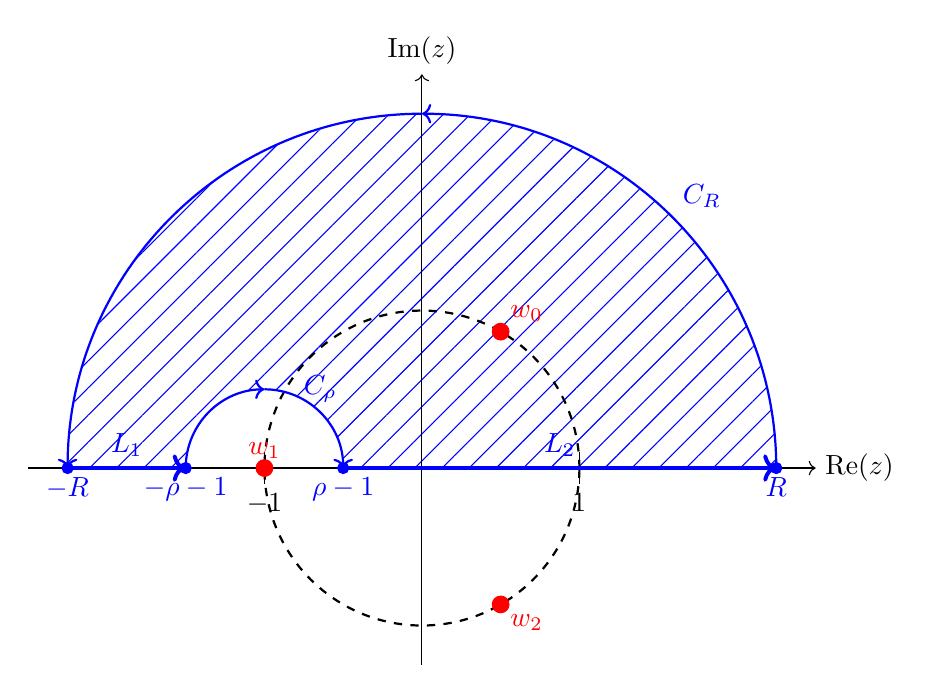
\begin{tikzpicture}[scale=2]
				\draw[white, pattern={Lines[angle=45,distance={12pt/sqrt(3)}]}, pattern color=blue] (2.25,0) arc (0:180:2.25) node[midway, above right] {};
				\filldraw[white] (-.5,0) arc (0:180:.5) node[midway, above right] {};
				% draw axes
				\draw[->] (-2.5,0) -- (2.5,0) node[right] {$\Re(z)$};
				\draw[->] (0,-1.25) -- (0,2.5) node[above] {$\Im(z)$};
				% draw unit circle
				\draw[dashed, thick] (1,0) arc (0:360:1) node[] {};
				%Take Coordinates
				\draw[] (1,.1)--(1,-.1) node[below] {$1$};
				\draw[] (-1,.1)--(-1,-.1) node[below] {$-1$};
				% solutions of z^3+1=0
				\filldraw[red] ({1/2},{sqrt(3)/2}) circle (1.5pt) node[anchor=south west] {$w_0$};
				\filldraw[red] (-1,0) circle (1.5pt) node[anchor=south] {$w_1$};
				\filldraw[red] ({1/2},-{sqrt(3)/2}) circle (1.5pt) node[anchor=north west] {$w_2$};
				
				% add arrow
				%\draw[->] (0,0) -- (1,1) node[midway, above left] {};
				% draw point
				\filldraw[blue] (2.25,0) circle (1pt) node[anchor=north] {$R$};
				\filldraw[blue] (-2.25,0) circle (1pt) node[anchor=north] {$-R$};
				\filldraw[blue] (-.5,0) circle (1pt) node[anchor=north] {$\rho-1$};
				\filldraw[blue] (-1.5,0) circle (1pt) node[anchor=north] {$-\rho-1$};
				
				\draw[line width=0.5mm, ->, thick, blue] (2.25,0) arc (0:90:2.25) node[midway, above right] {$C_R$};
				\draw[line width=0.5mm, ->, thick, blue] (0,2.25) arc (90:180:2.25) node[midway, left] {};
				\draw[line width=0.5mm, blue, ->] (-2.25,0) -- (-1.5,0) node[midway, above] {$L_1$};
				\draw[line width=0.5mm, blue, ->] (-.5,0) -- (2.25,0) node[midway, above] {$L_2$};
				
				\draw[line width=0.5mm, <-, thick, blue] (-.5,0) arc (0:90:.5) node[midway, above] {$C_\rho$};
				\draw[line width=0.5mm, <-, thick, blue] (-1,.5) arc (90:180:.5) node[midway, left] {};
			\end{tikzpicture}
		\end{center}
		demonstrate the following improper integral:\[
		\int_{-\infty}^{\infty}\frac{1}{x^3+1}\ dx=\frac{\pi}{\sqrt{3}}.
		\]
		\begin{proof}[\sol]
			Let $\displaystyle f(z):=\frac{1}{z^3+1}=\frac{1}{(z+1)(z-e^{\pi i/3})(z-e^{\pi 5i/3})}$. Then
			\begin{align*}
				\int_{-\infty}^{\infty}\frac{1}{x^3+1}\ dx&=2\pi i\res(f,w_0)+\pi i\res(f,w_1)\\
				&=2\pi i\cdot\frac{1}{3}\cdot\of{-\frac{1}{2}-\frac{\sqrt{3}}{2}i}+\frac{\pi i}{3}\\
				&=-\frac{\pi i}{3}+\frac{\sqrt{3}\pi}{3}+\frac{\pi i}{3}\\
				&=\frac{\pi}{\sqrt{3}}.
			\end{align*}
			Consider a path $C:=C_R+L_1+C_\rho+L_2$ where \begin{align*}
				C_R&: z(\theta)=Re^{i\theta}\quad(\theta\in[0,\pi]),\\
				L_1&: [-R,-\rho-1],\\
				L_2&: [\rho-1,R],\\
				C_\rho&: z(t)=\rho e^{i(\pi-t)}\quad(t\in[0,\pi]).
			\end{align*} Then $\oint_C f(z)\ dz=0$ by the Cauchy-Goursat Theorem. Consider \[
			0=\oint_C f(z)\ dz=\underbrace{\int_{C_R}f(z)\ dz}_{=(1)}+\underbrace{\int_{L_1\cup L_2}f(z)\ dz}_{=(2)}+\underbrace{\int_{C_\rho}f(z)\ dz}_{=(3)}
			\] \begin{enumerate}[(1)]
				\item Note that $\abs{f(z)}=\abs{\frac{1}{z^3+1}}\leq\frac{1}{\abs{z}^3+1}\frac{1}{R^3+1}=:M_R\to 0$ as $R\to\infty$. So \[
				\lim\limits_{R\to\infty}\int_{C_R}f(z)\ dz=0
				\] by Jordan's Lemma.
				\item \begin{align*}
					\int_{L_1\cup L_2}f(z)\ dz
					&=\int_{-R}^{-\rho-1}\frac{1}{x^3+1}\ dx+\int_{\rho-1}^{R}\frac{1}{x^3+1}\ dx\\
					&\to \int_{-\infty}^{\infty}\frac{1}{x^3+1}dx\quad\text{as}\quad\begin{cases}
						R\to\infty,\\
						\rho\to 0.
					\end{cases}
				\end{align*}
				\item Note that \begin{align*}
					f(z)=\frac{1}{z^3+1}&=\frac{1}{z+1}\of{arg1}\\
					&=\frac{1}{z}+\of{i+\frac{1}{2!}i^2z+\frac{1}{3!}i^3z^2+\cdots}\\
					&=\frac{1}{z}+g(z),
				\end{align*} where $\displaystyle g(z)=\sum_{n=0}^\infty \frac{1}{(n+1)!}i^{n+1}z^n$ is analytic at $z=0$. Consider \[
				\int_{C_\rho}f(z)e^{iz}\ dz=\underbrace{\int_{C_\rho}\frac{1}{z}\ dz}_{=\text{(a)}}+\underbrace{\int_{C_\rho} g(z)\ dz}_{=\text{(b)}}.
				\] \begin{enumerate}
					\item \[
					\int_{C_\rho}\frac{1}{z}\ dz=\int_0^{\pi}\frac{1}{\rho e^{i(\pi-t)}}\cdot i\rho e^{i(\pi-t)}(-1)\ dt=-i\int_0^{\pi}\ dt=-\pi i.
					\]
					\item Since $\exists M:\abs{g(z)}\leq M$ as $\abs{z}\leq\rho_0$, we have \[
					\int_{C_\rho}g(z)\ dz\leq M\cdot \pi\rho\to 0\quad\text{as $\rho\to 0$}.
					\]
				\end{enumerate}
			\end{enumerate}
			Therefore, by (1), (2) and (3), we obtain \[
			0=\lim\limits_{\substack{R\to\infty\\ \rho\to 0}}\oint_C f(z)e^{iz}\ dz=0+\int_{-\infty}^{\infty}\frac{\cos x}{x}dx + i\int_{-\infty}^{\infty}\frac{\sin x}{x}\ dx-\pi i,
			\] and so \[
			\int_{-\infty}^{\infty}\frac{\cos x}{x}dx + i\int_{-\infty}^{\infty}\frac{\sin x}{x}\ dx=0+\pi i\implies\boxed{\int_{-\infty}^{\infty}\frac{\sin x}{x}\ dx=\pi}.
			\]
		\end{proof}
		\item Referring to the figure below
		\begin{center}
			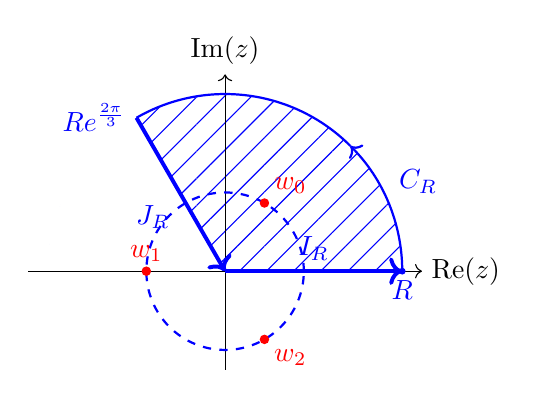
\begin{tikzpicture}[scale=1]
				\draw[white, pattern={Lines[angle=45,distance={12pt/sqrt(3)}]}, pattern color=blue] (2.25,0) arc (0:180:2.25) node[midway, above right] {};
				\filldraw[white] (0,0) -- (-2.25,0) arc (180:120:2.25) -- cycle;
				% draw axes
				\draw[->] (-2.5,0) -- (2.5,0) node[right] {$\Re(z)$};
				\draw[->] (0,-1.25) -- (0,2.5) node[above] {$\Im(z)$};
				% draw unit circle
				\draw[dashed, thick, blue] (1,0) arc (0:360:1) node[] {};
				% solutions of z^3+1=0
				\filldraw[red] ({1/2},{sqrt(3)/2}) circle (1.5pt) node[anchor=south west] {$w_0$};
				\filldraw[red] (-1,0) circle (1.5pt) node[anchor=south] {$w_1$};
				\filldraw[red] ({1/2},-{sqrt(3)/2}) circle (1.5pt) node[anchor=north west] {$w_2$};
				
				% add arrow
				%\draw[->] (0,0) -- (1,1) node[midway, above left] {};
				% draw point
				\filldraw[blue] (2.25,0) circle (1pt) node[anchor=north] {$R$};
				
				\draw[line width=0.5mm, ->, thick, blue] (2.25,0) arc (0:45:2.25) node[midway, above right] {$C_R$};
				\draw[line width=0.5mm, -, thick, blue] ({2.25*sqrt(2)/2},{2.25*sqrt(2)/2}) arc (45:120:2.25) node[left] {$\displaystyle Re^{\frac{2\pi}{3}}$};
				\draw[line width=0.5mm, blue, ->] (-{2.25*1/2},{2.25*sqrt(3)/2}) -- (0,0) node[midway, below left] {$J_R$};
				\draw[line width=0.5mm, blue, ->] (0,0) -- (2.25,0) node[midway, above] {$I_R$};
				
				%\draw[line width=0.5mm, <-, thick, blue] (-.5,0) arc (0:90:.5) node[midway, above] {$C_\rho$};
				%\draw[line width=0.5mm, <-, thick, blue] (-1,.5) arc (90:180:.5) node[midway, left] {};
			\end{tikzpicture}
		\end{center}
		demonstrate the following improper integral:\[
		\int_{0}^{\infty}\frac{1}{x^3+1}\ dx=\frac{2\pi}{3\sqrt{3}}.
		\]
	\end{enumerate}\begin{proof}[\sol]
		Firstly, let's find the isolated singularities (poles) of $f(z)=\frac{1}{z^3+1}$.
		
		Setting the denominator $z^3+1$ equal to zero, we find that $z^3 = -1$ which gives us the roots $z = w_k = \exp\left(\frac{i (2k + 1)\pi}{3}\right)$ for $k = 0, 1, 2$.
		
		Let's calculate the residue at each $w_k$.
		
		The residue Res($f(z); w_k$) of $f(z)$ at the pole $w_k$ is defined as the coefficient of $(z-w_k)^{-1}$ in the Laurent series of $f(z)$ centered at $w_k$.
		
		Here, we have a simple pole, so we can use the following formula for the residue at $w_k$:
		
		Res
		(
		�
		(
		�
		)
		;
		�
		�
		)
		=
		lim
		⁡
		�
		→
		�
		�
		(
		�
		−
		�
		�
		)
		�
		(
		�
		)
		Res(f(z);w 
		k
		​
		)=lim 
		z→w 
		k
		​
		
		​
		(z−w 
		k
		​
		)f(z)
		
		So we have:
		
		$\text{Res}(f(z); w_0) = \lim_{z\to w_0} (z - w_0) f(z)$
		$\text{Res}(f(z); w_1) = \lim_{z\to w_1} (z - w_1) f(z)$
		$\text{Res}(f(z); w_2) = \lim_{z\to w_2} (z - w_2) f(z)$
		Solving each, we find:
		
		$\text{Res}(f(z); w_0) = \lim_{z\to w_0} (z - w_0) \frac{1}{z^3+1} = \frac{1}{3(w_0^2 - w_0 w_1 - w_0 w_2)}$
		$\text{Res}(f(z); w_1) = \lim_{z\to w_1} (z - w_1) \frac{1}{z^3+1} = \frac{1}{3(w_1^2 - w_1 w_0 - w_1 w_2)}$
		$\text{Res}(f(z); w_2) = \lim_{z\to w_2} (z - w_2) \frac{1}{z^3+1} = \frac{1}{3(w_2^2 - w_2 w_0 - w_2 w_1)}$
		But since $w_0$, $w_1$ and $w_2$ are roots of the equation $z^3 = -1$, we know that $w_0 + w_1 + w_2 = 0$ and $w_0 w_1 + w_0 w_2 + w_1 w_2 = 0$ (from Vieta's formulas). Hence the residues at each singularity are:
		
		$\text{Res}(f(z); w_0) = -\frac{1}{3 w_0}$
		$\text{Res}(f(z); w_1) = -\frac{1}{3 w_1}$
		$\text{Res}(f(z); w_2) = -\frac{1}{3 w_2}$
		
		
		
		
		User
		demonstrate the following improper integral:\[
		\int_{0}^{\infty}\frac{1}{x^3+1}\ dx=\frac{2\pi}{3\sqrt{3}}.
		\]
		ChatGPT
		Sure, let's solve the integral using the method of contour integration.
		
		Let's consider the contour integral of $f(z) = \frac{1}{z^3 + 1}$ around a keyhole contour $\Gamma$ which starts from the positive real axis, encircles the origin in the positive direction, returns along the negative real axis, and then circles back to the positive real axis around a semicircular arc in the upper half-plane. We know that $f(z)$ has poles at $w_0$, $w_1$, and $w_2$.
		
		As per the Residue theorem, the integral of $f(z)$ around this contour is $2\pi i$ times the sum of the residues at its poles within the contour. Here, only $w_0$ and $w_1$ are within the contour, so:
		
		$\oint_{\Gamma} f(z),dz = 2\pi i (\text{Res}(f(z); w_0) + \text{Res}(f(z); w_1)) = 2\pi i (-\frac{1}{3 w_0} -\frac{1}{3 w_1})$
		
		The keyhole contour integral can be split into four parts: $\int_{R}^{1/R}$, $\int_{C_R}$, $\int_{1/R}^{R}$, and $\int_{C_{1/R}}$, where $C_R$ and $C_{1/R}$ are the semicircular contours with radii $R$ and $1/R$, respectively. As $R\rightarrow\infty$ and $1/R\rightarrow 0$, the integrals over $C_R$ and $C_{1/R}$ vanish (since $|f(z)|$ approaches 0 faster than $1/R$ on $C_R$ and faster than $R$ on $C_{1/R}$), so we have:
		
		$\int_{0}^{\infty} f(x),dx - \int_{0}^{\infty} f(-x),dx = 2\pi i (-\frac{1}{3 w_0} -\frac{1}{3 w_1})$
		
		Since $f(x)$ is an even function, we have $\int_{0}^{\infty} f(x),dx = \int_{0}^{\infty} f(-x),dx$, and therefore:
		
		$2\int_{0}^{\infty} f(x),dx = 2\pi i (-\frac{1}{3 w_0} -\frac{1}{3 w_1})$
		
		This simplifies to:
		
		$\int_{0}^{\infty} \frac{1}{x^3 + 1},dx = \frac{\pi i}{3} (-\frac{1}{w_0} -\frac{1}{w_1})$
		
		Substituting $w_0=\exp\left(\frac{i\pi}{3}\right)$ and $w_1=\exp\left(-\frac{i\pi}{3}\right)$, we get:
	\end{proof}
	\newpage
	\item Demonstrate the following improper integral: \[
	\int_{-\infty}^\infty\frac{\sin x}{x^2+4x+5}\ dx=-\frac{\pi}{e}\sin 2.
	\] \begin{proof}[\sol]
		Let $f(z):=\displaystyle\frac{1}{z^2+4z+5}=\frac{1}{(z+2-i)}\cdot\frac{1}{(z+2+i)}$, and let $\displaystyle f(z)e^{iz}=\frac{\phi(z)}{z+2-i}$ with $\phi(z)=\displaystyle\frac{e^{iz}}{z+2+i}$. Here, $\phi$ is analytic at $z=-2+i$. Let $C:=C_R+I_R$:
		\begin{center}
			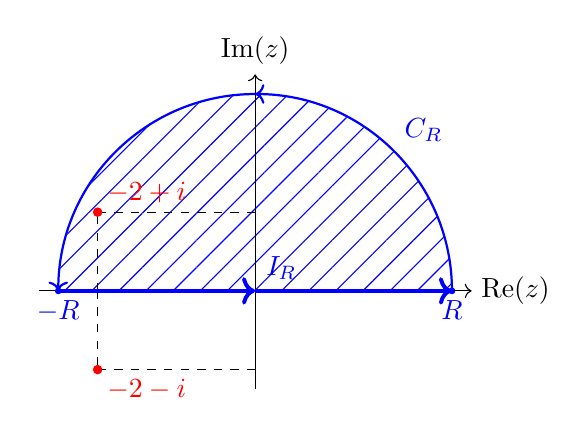
\begin{tikzpicture}[scale=1]
				\draw[white, pattern={Lines[angle=45,distance={12pt/sqrt(3)}]}, pattern color=blue] (2.5,0) arc (0:180:2.5) node[midway, above right] {};
				%\filldraw[white] (0,0) -- (-2.25,0) arc (180:120:2.25) -- cycle;
				\draw[-, dashed] (-2,0) -- (-2,-1);
				\draw[-, dashed] (-2,-1) -- (0,-1);
				\draw[-, dashed] (-2,0) -- (-2,1);
				\draw[-, dashed] (-2,1) -- (0,1);
				% draw axes
				\draw[->] (-2.75,0) -- (2.75,0) node[right] {$\Re(z)$};
				\draw[->] (0,-1.25) -- (0,2.75) node[above] {$\Im(z)$};
				% solutions of z^3+1=0
				\filldraw[red] (-2,1) circle (1.5pt) node[anchor=south west] {$-2+i$};
				\filldraw[red] (-2,-1) circle (1.5pt) node[anchor=north west] {$-2-i$};
				
				% add arrow
				%\draw[->] (0,0) -- (1,1) node[midway, above left] {};
				% draw point
				\filldraw[blue] (2.5,0) circle (1pt) node[anchor=north] {$R$};
				\filldraw[blue] (-2.5,0) circle (1pt) node[anchor=north] {$-R$};				
				
				
				\draw[line width=0.5mm, ->, thick, blue] (2.5,0) arc (0:90:2.5) node[midway, above right] {$C_R$};
				\draw[line width=0.5mm, ->, thick, blue] (0,2.5) arc (90:180:2.5) node[left] {};
				\draw[line width=0.5mm, blue, ->] (-2.5,0) -- (0,0) node[above right] {$I_R$};
				\draw[line width=0.5mm, blue, ->] (0,0) -- (2.5,0) node[] {};
				
				%\draw[line width=0.5mm, <-, thick, blue] (-.5,0) arc (0:90:.5) node[midway, above] {$C_\rho$};
				%\draw[line width=0.5mm, <-, thick, blue] (-1,.5) arc (90:180:.5) node[midway, left] {};
			\end{tikzpicture} then \[
			\Res_{z=-2+i}\left[f(z)e^{iz}\right]=\Res_{z=-2+i}\left[\frac{\phi(z)}{z+2-i}\right]=\phi(-2+i)=\frac{e^{i(-2+i)}}{2i}=\frac{e^{-2i}e^{-1}}{2i}=\frac{\cos(-2)+i\sin(-2)}{2e i}=\frac{\cos 2-i\sin 2}{2ei}.
			\]
		\end{center} Consider \[
		\oint_Cf(z)e^{iz}\ dz=\underbrace{\int_{C_R}f(z)e^{iz}\ dz}_{=\text{(1)}}+\underbrace{\int_{I_R}f(z)e^{iz}\ dz}_{=\text{(2)}}.
		\]
		\begin{enumerate}[(1)]
			\item Note that $\abs{f(z)}=\abs{\frac{1}{z^2+4z+5}}\leq\frac{1}{\abs{z}^2+\abs{4z}+5}=\frac{1}{R^2+4R+5}\to 0$ as $R\to\infty$, and so \[
			\lim\limits_{R\to\infty}\int_{C_R}f(z)e^{iz}\ dz=0
			\] by Jordan's Lemma.
			\item \[
			\int_{I_R}f(z)e^{iz}\ dz=\int_{-R}^R\frac{1}{x^2+4x+5}\cos x\ dx+i\int_{-R}^R\frac{1}{x^2+4x+5}\sin x\ dx.
			\]
		\end{enumerate}
		\vspace{4pt}
		Therefore, by (1) and (2), \begin{align*}
			\lim\limits_{R\to\infty}\oint_C f(z)e^{iz}\ dz&=\int_{-\infty}^{\infty}\frac{1}{x^2+4x+5}\cos x\ dx+i\int_{-\infty}^{\infty}\frac{1}{x^2+4x+5}\sin x\ dx\\
			&=2\pi i\cdot\res\of{f(z)e^{iz}, -2+i}\quad\text{by Residue Theorem}\\
			&=2\pi i\cdot \frac{\cos 2-i\sin 2}{2ei}\\
			&=\frac{\pi\cos 2}{e}+i\of{-\frac{\pi\sin 2}{e}}.
		\end{align*} Hence \[
		\int_{-\infty}^\infty\frac{\sin x}{x^2+4x+5}\ dx=-\frac{\pi}{e}\sin 2.
		\]
	\end{proof}
	\item Demonstrate the following improper integral: \[
	\int_0^{\infty}\frac{x^2}{x^6+1}\ dx=\frac{\pi}{6}.
	\] \begin{proof}[\sol]
		Let $\displaystyle f(z):=\frac{z^2}{z^6+1}$. $e^{\frac{\pi i}{6}}, e^{\frac{2\pi i}{3}},e^{\pi i}, e^{\frac{4\pi i}{3}},e^{\frac{5\pi i}{3}}, e^{2\pi i}$ \begin{align*}
			\res\of{f,w_0}&=\lim\limits_{z\to w_0}(z-w_0)f(z)=\lim\limits_{z\to w_0}\frac{z^3-z^2w_0}{z^6+1}=\lim\limits_{z\to w_0}\frac{3z^2-2zw_0}{6z^5}=\frac{w_0^2}{6w_0^5}=\frac{1}{6}w_0^{-3}=\frac{1}{6}\of{e^{\frac{\pi}{6}i}}^{-3}=\frac{1}{6}e^{-\frac{\pi}{2}i}\\
			\res\of{f,w_1}&=\frac{1}{6}w_1^{-3}=\frac{1}{6}\of{e^{\frac{3\pi}{6}i}}^{-3}=\frac{1}{6}e^{-\frac{3\pi}{2}i}\\
			\res\of{f,w_2}&=\frac{1}{6}w_2^{-3}=\frac{1}{6}\of{e^{\frac{5\pi i}{6}}}^{-3}=\frac{1}{6}e^{-\frac{5\pi}{2}i}.
		\end{align*}
		\begin{center}
			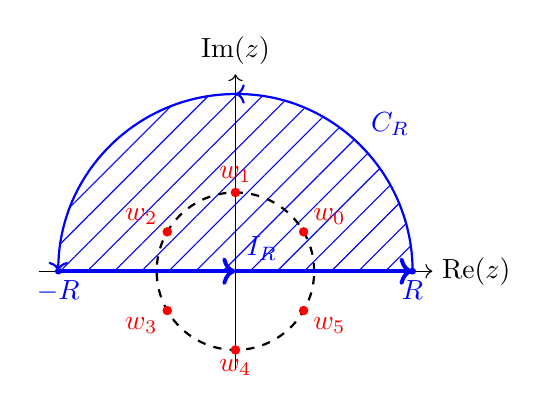
\begin{tikzpicture}[scale=1]
				\draw[white, pattern={Lines[angle=45,distance={12pt/sqrt(3)}]}, pattern color=blue] (2.25,0) arc (0:180:2.25) node[midway, above right] {};
				%\filldraw[white] (-.5,0) arc (0:180:.5) node[midway, above right] {};
				% draw axes
				\draw[->] (-2.5,0) -- (2.5,0) node[right] {$\Re(z)$};
				\draw[->] (0,-1.25) -- (0,2.5) node[above] {$\Im(z)$};
				% draw unit circle
				\draw[dashed, thick] (1,0) arc (0:360:1) node[] {};
				% solutions of z^6+1=0
				\foreach \angle/\label [count=\k from 0] in {30/$w_0$, 90/$w_1$, 150/$w_2$, 210/$w_3$, 270/$w_4$, 330/$w_5$} {
					\coordinate (z\k) at (\angle:1);
					\draw[fill, red] (z\k) circle (1.5pt) node[anchor={\angle-180}, shift={(0,0)}] {\label};
				}
				
				% add arrow
				%\draw[->] (0,0) -- (1,1) node[midway, above left] {};
				% draw point
				\filldraw[blue] (2.25,0) circle (1pt) node[anchor=north] {$R$};
				\filldraw[blue] (-2.25,0) circle (1pt) node[anchor=north] {$-R$};		
				
				\draw[line width=0.5mm, ->, thick, blue] (2.25,0) arc (0:90:2.25) node[midway, above right] {$C_R$};
				\draw[line width=0.5mm, ->, thick, blue] (0,2.25) arc (90:180:2.25) node[left] {};
				\draw[line width=0.5mm, blue, ->] (-2.25,0) -- (0,0) node[above right] {$I_R$};
				\draw[line width=0.5mm, blue, ->] (0,0) -- (2.25,0) node[] {};				
			\end{tikzpicture}
		\end{center}
		\begin{align*}
			\int_{-\infty}^{\infty}\frac{x^2}{x^6+1}\ dx&=2\pi i\sum_{i=0}^3\res(f,w_i)\\
			&=2\pi i\cdot\frac{1}{6}\cdot\of{e^{-\frac{\pi}{2}i}+e^{-\frac{3\pi}{2}i}+e^{-\frac{5\pi}{2}i}}\\
			&=2\pi i\cdot\frac{1}{6}\cdot\of{(-i)+(i)+(-i)}\\
			&=\frac{\pi}{3}.
		\end{align*} Hence \[
		\int_0^{\infty}\frac{x^2}{x^6+1}\ dx=\frac{1}{2}\cdot\frac{\pi}{3}=\frac{\pi}{6}.
		\]
	\end{proof}
	\item 
	Using the Rouché's theorem, demonstrate the number of roots the equation $z^3 - z - 4 = 0$ has within the domain $\set{z\in\C:\abs{z}<2}.$ 
	\begin{tcolorbox}[colback=white,colframe=thmcolor,arc=5pt,title={\color{white}\bf Rouch\'{e}'s Theorem}]
		\begin{theorem*}
			Let \begin{enumerate}[(1)]
				\item Let $D$ be the region enclosed by simply closed curve $\gamma$;
				\item $f$ and $g$ be complex-valued function  which are holomorphic in $D$
				\item $\abs{g(z)}<\abs{f(z)}$ on $\gamma$.
			\end{enumerate} Then $f$ and $f+g$ have the same number of zeros in $D$ counted up to multiply.
	\end{theorem*}
	\end{tcolorbox}
	\begin{proof}[\sol]
		Let $f(z)+g(z)=0$ where $f(z)=z^3$ and $g(z)=-z-4$. For $\abs{z}=2$, we have \begin{align*}
			\abs{f(z)}&=\abs{z^3}=8,\\
			\abs{g(z)}&=\abs{-z-4}=6.
		\end{align*} Then $\abs{f(z)}>\abs{g(z)}$ for all $z$ with $\abs{z}=2$. Since $f(z)=z^3$ has 3 roots in the complex plane, so $f(z)+g(z)=z^3-z-4$ must also have 3 roots in the disc $\abs{z}<2$. Hence, by Rouch\'{e}'s Theorem, the equation $z^3-z-4=0$ has three roots within the domain $\abs{z}<2$. 
	\end{proof}
	\item \begin{proof}[\sol]
		Find the conformal mapping that sends the region $D=\set{re^{i\theta}\in\C:0\leq r<1,\ 0<\theta<\pi/2}$ to the open disc $U=\set{z\in\C:\abs{z}<1}$
		[Hint: It can be created by composing functions $f_1(z)$ to $f_4(z)$. The function $f_2(z)$ is the inverse of a conformal mapping that sends the right half-plane to the interior of the unit disc. Also, two among $f_1(z)$ to $f_4(z)$ are the function $z\mapsto z^2$.]
		
		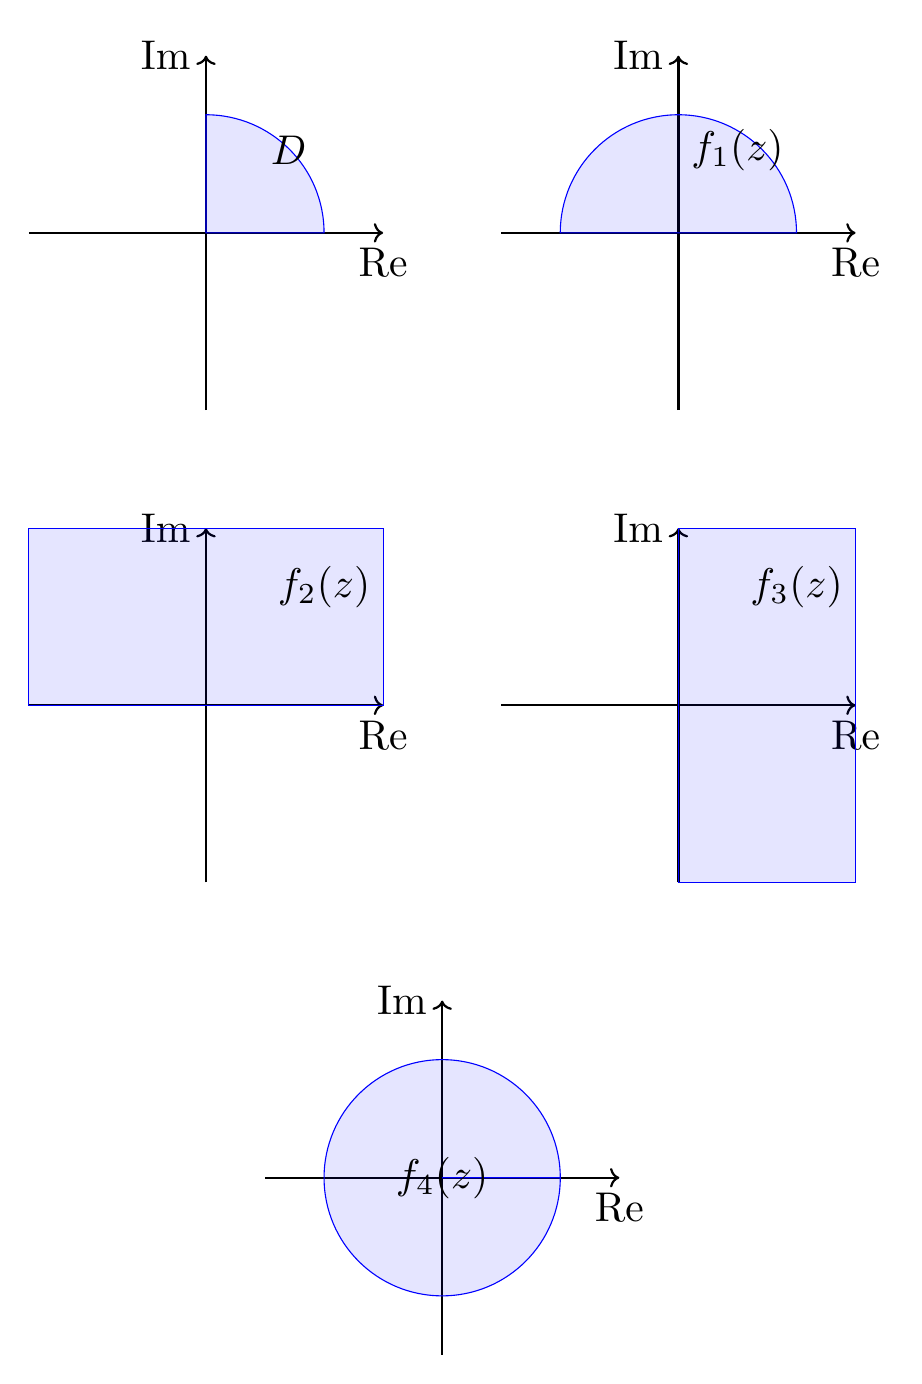
\begin{tikzpicture}[scale=1.5, transform shape]
			
			\draw[thick,->] (-1.5,0) -- (1.5,0) node[below] {$\Re$}; % x-axis
			\draw[thick,->] (0,-1.5) -- (0,1.5) node[left] {$\Im$}; % y-axis
			
			\draw[color=blue, fill=blue, fill opacity=0.1] (0,0) -- (0:1cm) arc (0:90:1cm) -- cycle; % quarter of unit disc
			\node at (0.7,0.7) {$D$};
			
			\begin{scope}[xshift=4cm]
				\draw[thick,->] (-1.5,0) -- (1.5,0) node[below] {$\Re$}; % x-axis
				\draw[thick,->] (0,-1.5) -- (0,1.5) node[left] {$\Im$}; % y-axis
				
				\draw[color=blue, fill=blue, fill opacity=0.1] (0,0) -- (0:1cm) arc (0:180:1cm) -- cycle; % upper half disc
				\node at (0.5,0.7) {$f_1(z)$};
			\end{scope}
			
			\begin{scope}[yshift=-4cm]
				\draw[thick,->] (-1.5,0) -- (1.5,0) node[below] {$\Re$}; % x-axis
				\draw[thick,->] (0,-1.5) -- (0,1.5) node[left] {$\Im$}; % y-axis
				
				\draw[color=blue, fill=blue, fill opacity=0.1] (-1.5,0) -- (1.5,0) -- (1.5,1.5) -- (-1.5,1.5) -- cycle; % upper half plane
				\node at (1,1) {$f_2(z)$};
			\end{scope}
			
			\begin{scope}[xshift=4cm, yshift=-4cm]
				\draw[thick,->] (-1.5,0) -- (1.5,0) node[below] {$\Re$}; % x-axis
				\draw[thick,->] (0,-1.5) -- (0,1.5) node[left] {$\Im$}; % y-axis
				
				\draw[color=blue, fill=blue, fill opacity=0.1] (0,-1.5) -- (0,1.5) -- (1.5,1.5) -- (1.5,-1.5) -- cycle; % right half plane
				\node at (1,1) {$f_3(z)$};
			\end{scope}
			
			\begin{scope}[xshift=2cm, yshift=-8cm]
				   \draw[thick,->] (-1.5,0) -- (1.5,0) node[below] {$\Re$}; % x-axis
				\draw[thick,->] (0,-1.5) -- (0,1.5) node[left] {$\Im$}; % y-axis
				
				\draw[color=blue, fill=blue, fill opacity=0.1] (0,0) -- (0:1cm) arc (0:360:1cm) -- cycle; % unit disc
				\node at (0,0) {$f_4(z)$};
			\end{scope}
		
	\end{tikzpicture}
	\end{proof}
	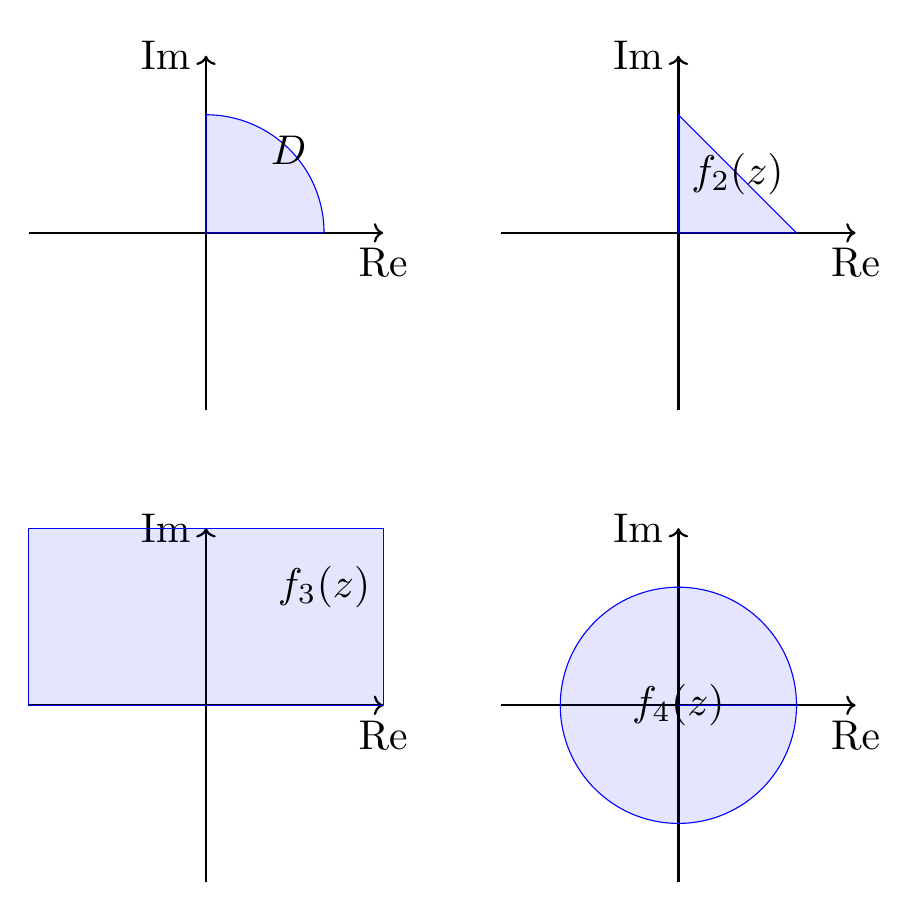
\begin{tikzpicture}[scale=1.5, transform shape]
		
		\draw[thick,->] (-1.5,0) -- (1.5,0) node[below] {$\Re$}; % x-axis
		\draw[thick,->] (0,-1.5) -- (0,1.5) node[left] {$\Im$}; % y-axis
		
		\draw[color=blue, fill=blue, fill opacity=0.1] (0,0) -- (0:1cm) arc (0:90:1cm) -- cycle; % quarter of unit disc
		\node at (0.7,0.7) {$D$};
		
		\begin{scope}[xshift=4cm]
			\draw[thick,->] (-1.5,0) -- (1.5,0) node[below] {$\Re$}; % x-axis
			\draw[thick,->] (0,-1.5) -- (0,1.5) node[left] {$\Im$}; % y-axis
			
			\draw[color=blue, fill=blue, fill opacity=0.1] (0,0) -- (1,0) -- (0,1) -- cycle; % triangle in the first quadrant
			\node at (0.5,0.5) {$f_2(z)$};
		\end{scope}
		
		\begin{scope}[yshift=-4cm]
			\draw[thick,->] (-1.5,0) -- (1.5,0) node[below] {$\Re$}; % x-axis
			\draw[thick,->] (0,-1.5) -- (0,1.5) node[left] {$\Im$}; % y-axis
			
			\draw[color=blue, fill=blue, fill opacity=0.1] (-1.5,0) -- (-1.5,1.5) -- (1.5,1.5) -- (1.5,0) -- cycle; % right half plane
			\node at (1,1) {$f_3(z)$};
		\end{scope}
		
		\begin{scope}[xshift=4cm, yshift=-4cm]
			\draw[thick,->] (-1.5,0) -- (1.5,0) node[below] {$\Re$}; % x-axis
			\draw[thick,->] (0,-1.5) -- (0,1.5) node[left] {$\Im$}; % y-axis
			
			\draw[color=blue, fill=blue, fill opacity=0.1] (0,0) -- (0:1cm) arc (0:360:1cm) -- cycle; % unit disc
			\node at (0,0) {$f_4(z)$};
		\end{scope}
		
	\end{tikzpicture}\\
	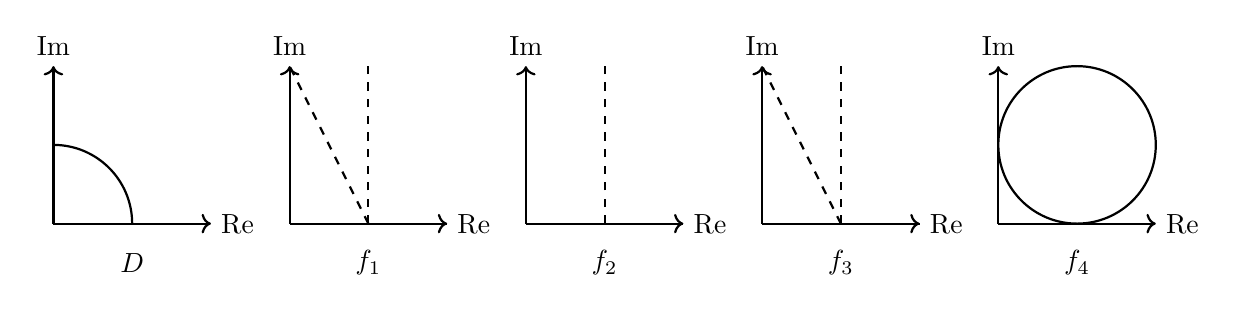
\begin{tikzpicture}
		
		% Define the scale for each of the plots
		\def\s{1}
		
		% Define the labels for each transformation
		\def\labels{{"$D$", "$f_1$", "$f_2$", "$f_3$", "$f_4$", "$U$"}}
		
		% Plot each stage of the transformation
		\foreach \i in {0,...,4} {
			
			% Draw the axes
			\draw [->,thick] (\i*3*\s,0) -- ++(2*\s,0) node [right] {$\Re$};
			\draw [->,thick] (\i*3*\s,0) -- ++(0,2*\s) node [above] {$\Im$};
			
			% Draw the region for this stage of the transformation
			\ifnum\i=0
			% Draw the quarter-disc for D
			\draw [thick] (\i*3*\s+1*\s,0) arc (0:90:1*\s);
			\draw [thick] (\i*3*\s,0) -- (\i*3*\s+1*\s,0);
			\draw [thick] (\i*3*\s,0) -- (\i*3*\s,1*\s);
			\else
			\ifnum\i=4
			% Draw the full disc for U
			\draw [thick] (\i*3*\s+1*\s,1*\s) circle (1*\s);
			\else
			\ifnum\i=2
			% Draw the half plane for f_2
			\draw [thick] (\i*3*\s,0) -- (\i*3*\s+2*\s,0);
			\draw [thick, dashed] (\i*3*\s+1*\s,0) -- (\i*3*\s+1*\s,2*\s);
			\else
			% Draw the plane without non-positive real axis for f_3
			\draw [thick] (\i*3*\s,0) -- (\i*3*\s+2*\s,0);
			\draw [thick, dashed] (\i*3*\s+1*\s,0) -- (\i*3*\s+1*\s,2*\s);
			\draw [thick, dashed] (\i*3*\s+1*\s,0) -- (\i*3*\s,2*\s);
			\fi
			\fi
			\fi
			
			% Draw the label for this stage of the transformation
			\node at (\i*3*\s+1*\s,-0.5*\s) {\pgfmathparse{\labels[\i]}\pgfmathresult};
		}
		
	\end{tikzpicture}
	
	\newpage
	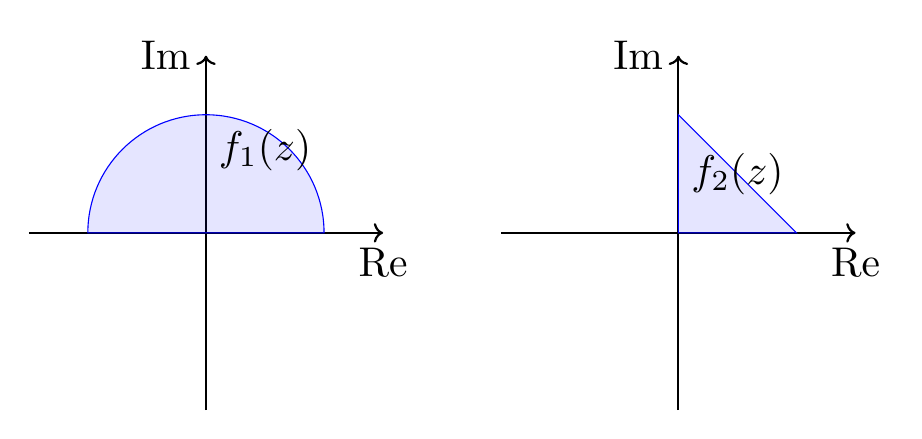
\begin{tikzpicture}[scale=1.5, transform shape]
		\begin{scope}[xshift=-2cm]
			\draw[thick,->] (-1.5,0) -- (1.5,0) node[below] {$\Re$}; % x-axis
			\draw[thick,->] (0,-1.5) -- (0,1.5) node[left] {$\Im$}; % y-axis
			
			\draw[color=blue, fill=blue, fill opacity=0.1] (0,0) -- (0:1cm) arc (0:180:1cm) -- cycle; % upper half disc
			\node at (0.5,0.7) {$f_1(z)$};
		\end{scope}
		\\
		\begin{scope}[xshift=2cm]
			\draw[thick,->] (-1.5,0) -- (1.5,0) node[below] {$\Re$}; % x-axis
			\draw[thick,->] (0,-1.5) -- (0,1.5) node[left] {$\Im$}; % y-axis
			
			\draw[color=blue, fill=blue, fill opacity=0.1] (0,0) -- (1,0) -- (0,1) -- cycle; % triangle in the first quadrant
			\node at (0.5,0.5) {$f_2(z)$};
		\end{scope}
	\end{tikzpicture}
	\item \begin{proof}[\sol]
		content...
	\end{proof}
\end{enumerate}

\footer{Department of Information Security, Cryptography and Mathematics\\
	College of Science and Technology\\
	Kookmin University}
\end{document}
